% Chapter 4

\chapter{Experiments}
\label{Chapter4}

In order to assess the quality of the proposed methodology, described in Section
\ref{sec:method}, we tested it on several commonly adopted benchmarks and against
different baselines that are detailed in the following sections.

\section{Datasets}
\label{subsec:datasets}

The experiments were conducted on five real-world applications datasets, namely:
AIDS \cite{Weislow19041989}, CAS\footnote{http://cheminformatics.org/datasets/bursi/},
CPDB \cite{journals/jcisd/HelmaCKR04}, GDD \cite{dobson2003}, and NCI1 \cite{journals/kais/WaleWK08}.
All these datasets contains chemical and molecular particles encoded in graph form,
all the nodes are labelled and none have self loops, that is an edge going out
and into the same node.
The AIDS Antiviral Screen dataset contains chemical compounds, labelled according to
their antiviral activity; CAS and CPDB are dataset of mutagenic
compounds; NCI1 consists of chemical compounds screened for activity against 
non-small lung cancer cells; GDD is composed of X-ray crystal structures of
proteins represented as graphs.
    \begin{table}[ht]
        \centering
        \begin{tabular}{|r|r|r|r|r|}
            \hline
            Dataset & n. of graphs & sample split & avg nodes & avg edges \\ \hline
            AIDS    & 1503         & 28.07        & 58.90     & 61.40     \\ \hline      
            CAS     & \textbf{4337} & 55.36        & 29.90     & 30.90     \\ \hline      
            CPDB    &  684         & 49.85        & 14.10     & 14.60     \\ \hline      
            GDD     & 1503         & 58.65        & 284.31    & \textbf{2862.63}   \\ \hline      
            NCI1    & 1503         & 50.04        & 29.87     & 32.30     \\ \hline      
        \end{tabular}
        \caption{Statistics about the datasets employed in the experiments: number
        of graphs, labels percentage among samples, average number of nodes, average
        number of edges.}
        \label{table:datasets}
    \end{table}

Some statistics about these datasets are reported in table~\ref{table:datasets},
from this data it is clear that the CAS and NCI1 datasets are the bigger ones
while the GDD holds the most complex graphs in terms of topography.
Furthermore the AIDS dataset turns out to be quite unbalanced in terms of labels
distribution \cite{rtesselli}.  

%----------------------------------------------------------------------------------------

\section{Experiments description}
\label{sec:description}

All the experiments exposed in this section consist in a nested k-fold
cross-validation routine.
The $k$ parameter of the cross-validation is fixed at 10 since this value
already provides good statistical significance while helping containing the bias
skewing during the training phase.
Moreover, the whole routine has been run ten times with ten different splits of the
data in order to mitigate the high variance derived during the testing phase due to the
chosen value of $k$.

\subsection{Baselines}
% what
The baseline method to which we compare our methodology is a grid search (\ref{subsubsec:grid})
employing the Support Vector Machine (Section \ref{subsubsec:svm}).
The kernels tested with this approach are:
\begin{itemize}
    \item $TCK_{ST}$ (Section \ref{subsec:context}) and the kernel resulting
        from the sum of $TCK_{ST}$ and $ODDK_{ST}$ (Section \ref{subsubsec:odd});
    \item $TCK_{ST+}$ (Section \ref{subsec:context}) and the sum of $TCK_{ST+}$
        and $ODDK_{ST+}$ (Section \ref{subsubsec:odd});
    \item $WLC$ (Section \ref{subsec:context}) and the sum of $WLC$ and $WL$
        (Section \ref{subsubsec:fs}).
\end{itemize}

% how &  why
This method perform a standard hyper-parameter selection using an exhaustive search
on a finite subset of the parameter space deriving from the composition of the
respective spaces of the kernel function and kernel machine.
The choice of kernels is such that we can compare the performances over a single
kernel function and the implicit combination, i.e. the sum, of the the feature
spaces of two different functions respectively.
This combination is reproposed in the experiments employing the new method altough
in an explicit fashion.

Each kernel function has been used to train a SVM classifier whose $C$ parameter
was validated on the set $\{10^{-3},10^{-2},\dots,10^3\}$.
The kernel functions parameter where validated on the following sets:
\begin{itemize}
    \item for the kernels derived from the $ODD$ framework:
    \begin{itemize}
        \item $h=\{1,\dots,10\}$ and 
        \item $\lambda=\{0.1, 0.5, 0.8, 0.9, 1.0, 1.1, 1.2, 1.3, 1.4, 1.5, 1.8\}$,
    \end{itemize}
    \item for the kernels derived from the $WL$ framework:
    \begin{itemize}
        \item $h=\{1,\dots,10\}$.
    \end{itemize}
\end{itemize}
The parameter sets both for the kernels and the classifier were taken from \cite{rtesselli}.

Moreover, for the first combination of the list ($TCK_{ST}$ and $ODDK_{ST}$)
we compare our results against those in \cite{gmkl} which are:

\begin{itemize}
    \item $ODD-MKL$ kernel with EasyMKL as kernel machine, and
    \item $ODD_{ST}$ kernel with SVM as kernel machine.
\end{itemize}

These experiments perform a hyper-parameter selection employing both a single and 
a multiple kernel learning approach using two of the kernel function selected here.
In particular the experiments concerning the $ODD-MKL$ kernel use a setup similar to
our methodology while employing only the kernels computed from a single tuple of
parameters coming from the grid for each experiment.
The experiments carried on in \cite{gmkl} employ a slightly different parameter grid
than the one used here, namely the $h$ parameter of the $ODD-MKL$ and $ODDK_{ST}$ is
validated on the set $\{1,\dots,8\}$, the parameter $\lambda$ of the $ODDK_{ST}$ is 
validated on the set $\{0.5,0.6,\dots,1.6\}$ and the $C$ parameter of the SVM
is validated on the set $\{10^{-4},10^{-3},\dots,10^4\}$.

%Table \ref{table:baselines} describes the general structure of the experiments
%designed with this aim.
%
%\begin{table}[ht]
%    \centering
%    \begin{tabular}{|l|l|l|}
%        \hline
%        n. & method & kernels \\
%        \hline
%        4 & EasyMKL & $K$ and $K'$ \\
%        \hline
%        5 & EasyMKL & $K'$ \\
%        \hline
%        6 & EasyMKL & $K$ \\
%        \hline
%        7 & SVC & $K'$ \\
%        \hline
%        8 & SVC & $K'+K$ \\
%        \hline
%    \end{tabular}
%    \caption{Structure of the baseline experiments. Kernels $K$ and $K'$ refer
%    to the version without and with contexts for each combination respectively.
%    These kernels generated a set of matrices each, according to the hyper-parameters
%    grid, which were concatenated as a list to be given in input to EasyMKL or
%    given individually to an instance of the SVC. The expression $K + K'$ refers
%    to the fact that the two kernel were summed prior to be used.}
%    \label{table:baselines}
%\end{table}

\subsection{The proposed method}
\label{subsec:firstg}

These experiments aim to test the basic methodology proposed in Section \ref{sec:method},
in other words they implement the scheme in Figure \ref{fig:comp2}.
The kernels selected for this set of experiments are:
\begin{enumerate}
    \item the $ODDK_{ST}$ (Section \ref{subsubsec:odd}) and $TCK_{ST}$ (Section \ref{subsec:context}) graph kernels,
    \item the $ODDK_{ST+}$ (Section \ref{subsubsec:odd}) and $TCK_{ST+}$ (Section \ref{subsec:context}) graph kernels,
    \item the $WL$ (Section \ref{subsubsec:fs}) fast subtree and $WLC$ (Section \ref{subsec:context}) graph kernels.
\end{enumerate}
The kernel machine employed is EasyMKL, see Section \ref{subsec:easymkl}.

The kernels derived from the $ODD$ framework are calculated according to a parameters grid
composed from the sets:
\begin{itemize}
    \item $h=\{1,\dots,10\}$ and 
    \item $\lambda=\{0.1, 0.5, 0.8, 0.9, 1.0, 1.1, 1.2, 1.3, 1.4, 1.5, 1.8\}$,
\end{itemize}
both sets are taken from \cite{rtesselli}.
To calculate the kernels derived from the $WL$ framework a grid corresponding to
the set $h=\{1,\dots,10\}$ is employed, were $h$ is the only hyper-parameter of
the $WL$ kernels, see Section \ref{subsubsec:fs}.

The hyper-parameter selection is done only for the kernel machine and refers
to the parameter grid derived from the set $\Lambda=\{0.0, 0.1,\dots,1.0\}$, i.e. the
only hyper-paramter of the EasyMKL algorithm.

\subsection{The proposed method with kernel orthogonalization}
\label{subsec:secondg}
%Section \ref{subsec:features}.

% add more motivations behind these experiments.
The kernel combinations selected for these experiments are the same of Section \ref{subsec:firstg}.
%\begin{enumerate}
%    \item the $ODDK_{ST}$ (Section \ref{subsubsec:odd}) and $TCK_{ST}$ (Section \ref{subsec:context}) graph kernels,
%    \item the $ODDK_{ST+}$ (Section \ref{subsubsec:odd}) and $TCK_{ST+}$ (Section \ref{subsec:context}) graph kernels,
%    \item the $WL$ (Section \ref{subsubsec:fs}) fast subtree and $WLC$ (Section \ref{subsec:context}) graph kernels.
%\end{enumerate}

%\begin{table}[ht]
%    \centering
%    \begin{tabular}{|l|l|l|}
%        \hline
%        n. & method & kernels \\
%        \hline
%        1 & EasyMKL & $K$ and $K'$ \\
%        \hline
%        2 & EasyMKL & $K'$ \\
%        \hline
%        3 & EasyMKL & $K$ \\
%        \hline
%    \end{tabular}
%    \caption{Structure of the main experiments. Kernels $K$ and $K'$ refer
%    to the version without and with contexts for each combination respectively.
%    These kernels generated a set of matrices each, according to the technique
%    described in Section \ref{subsec:features} which were concatenated as a list
%    to be given in input to EasyMKL.}
%    \label{table:structure}
%\end{table}

These experiments model the methodology proposed in Section \ref{subsec:features}.
The set of kernel matrices has been pre-computed for each one of the possible combinations
of a parameter grid thus defined:

\begin{itemize}
    \item for the kernels derived from the $ODD$ framework:
    \begin{itemize}
        \item $h=\{1,\dots,10\}$
        \item the $\lambda$ parameter was fixed to 1 for the reasons explained in \ref{subsec:features}
    \end{itemize}
    \item for the kernels derived from the $WL$ the parameter $h$ was set to 10
        given the nature of the orthogonalization applied to this kernel (DRAFT: explain).
\end{itemize}
The parameter sets both for the kernels and the classifier were taken from \cite{rtesselli}.
For all the experiments, the $\Lambda$ parameter of EasyMKL has been
validated on the set $\{0.0, 0.1,\dots,1.0\}$ during the cross-validation
routine.

\paragraph{The case of the GDD dataset:}
\label{par:gdd}
confirming the experience reported in \cite{rtesselli}, while working with the GDD
dataset and the $ODD$ kernels we had to limit the $h$ hyper-parameter to the set
$\{1,2,3\}$ because for heights greater than 3 the computational times of the
kernel matrices became prohibitive, due to the high complexity and magnitude
of the data structures contained in this dataset.

%----------------------------------------------------------------------------------------

\section{Results and discussion}
\label{sec:results}

\subsection{Space resources requirements}
Given the large number of kernel matrices involved in the combination exepriments
we would like to detail the space resources requirements that these experiments
have when the basic methodology (\ref{subsec:firstg}) and the improved one (\ref{subsec:secondg})
are applied.
Table \ref{table:mem1} shows the data obtained in the first case while \ref{table:mem2} shows
the data obtained after applying the kernel orthogonalization strategy.
The data shown here only concerns the $ODD_{ST}$ and $TCK_{ST}$ kernels since for the 
other $ODD$-derived kernels the numbers were basically the same.
The $WL$ and $WLC$ kernel both generated the same amount of matrices in both cases
due to the variation in the parameter grids described above.

\begin{table}[ht]
    \centering\footnotesize
    \begin{tabular}{|l|l|r|r|r|r|r|r|}
        \hline
        n. & kernels & no. k. & AIDS & CAS & CPDB & GDD & NCI1 \\
        \hline
        4 & $TCK_{ST}$ and $ODD_{ST}$ & 220 & 10 GB & 56 GB & 5 GB & 3 GB & 48 GB \\
        \hline
        5 & $TCK_{ST}$ & 110 & 5 GB & 32 GB & 2 GB & 1 GB & 24 GB \\
        \hline
        6 & $ODD_{ST}$ & 110 & 5 GB & 32 GB & 2 GB & 1 GB & 24 GB \\
        \hline
    \end{tabular}
    \caption{\footnotesize The number of computed kernels matrices and the memory
    occupation in GigaBytes for each dataset during the experiments relative to
    Section \ref{subsec:firstg}.}
    \label{table:mem1}
\end{table}
\begin{table}[ht]
    \centering\footnotesize
    \begin{tabular}{|l|l|r|r|r|r|r|r|}
        \hline
        n. & kernels & no. k. & AIDS & CAS & CPDB & GDD & NCI1 \\
        \hline
        1 &  $TCK_{ST}$ and $ODD_{ST}$ & 130 & 5 GB & 34 GB & 3 GB & <2 GB & 29 GB \\
        \hline
        2 &  $TCK_{ST}$ & 65 & 3 GB & 19 GB & <2 GB & <1 GB & 17 GB \\
        \hline
        3 & $ODD_{ST}$ & 65 & 3 GB & 19 GB & <2 GB & <1 GB & 17 GB \\
        \hline
    \end{tabular}
    \caption{\footnotesize The number of computed kernels matrices and the memory
    occupation in GigaBytes for each dataset during the experiments relative to
    Section \ref{subsec:secondg}.}
    \label{table:mem2}
\end{table}

Time resources requirements being a part of the proposed improvements is given
in Section \ref{subsec:time_results}.

\subsection{Analysis of computational times}
\label{subsec:time_results}

The plot in figure~\ref{fig:times} shows the relation between the computation times
for the $ODD_{ST}\text{ and }TCK_{ST}$ kernels combination on the benchmark datasets,
using Algorithm \ref{alg:incremental} detailed in Section \ref{subsec:inc}.
See Section~\ref{subsec:datasets} for further details on the composition of each dataset.
From the data it is clear that the complexity of computing the kernel in an incremental
fashion does not grow with the number of kernels being computed.

\begin{figure}[ht]
    \centering
    \includegraphics[scale=0.5]{Figures/kernel_times_log2}
    \caption{Times in seconds required to compute the kernels $ODD_{ST}$ and 
    $TCK_{ST}$ incrementally and sequentially on a selection of datasets. Time
    scale is logarithmic for the sake of presentation.}
    \label{fig:times}
\end{figure}

We now present an analysis of the computational time performances of our methodology
compared to the two baselines. To keep the results comparable we are here considering
only the results obtained by experiments no. 2, 6, and 8; this choice stem from the fact
that these experiments employ the same kernel function with three different methods.

\begin{figure}[ht]
    \centering
    \includegraphics[scale=0.7]{Figures/total_times}
    \caption{(DRAFT: this plot will be replicated for each one of the kernels combination)
        Plot of the times required to compute a full nested
        10-fold cross-validation on the benchmark datasets.
        The data shown here refers to experiments 2 (cyan), 6 (magenta) and 8 (yellow)
        i.e. with the kernel $TCK_{ST}$.
    }
    \label{fig:datasetstimes}
\end{figure}

As one can see from Figure \ref{fig:datasetstimes}, our method performs generally
better or has comparable performances with respect to the single-kernel approach.
The only case where our method fares worse is with the GDD dataset and this can be
ascribed to the particular case which it represents, that is, due to the parameters
set limitation in this case we had way less matrices than we should have had and
this positively affects the single kernel method while being of no relevance for
EasyMKL, less influenced by the number of input matrices.
From this data we can finally conclude that our methodology is more susceptible
to dataset dimension variation (i.e. the number of records) while the single-kernel
method is ideed influenced by the same measure but it is even more influenced by
the dimensions of the parameters grid.

\begin{figure}[ht]
    \centering
    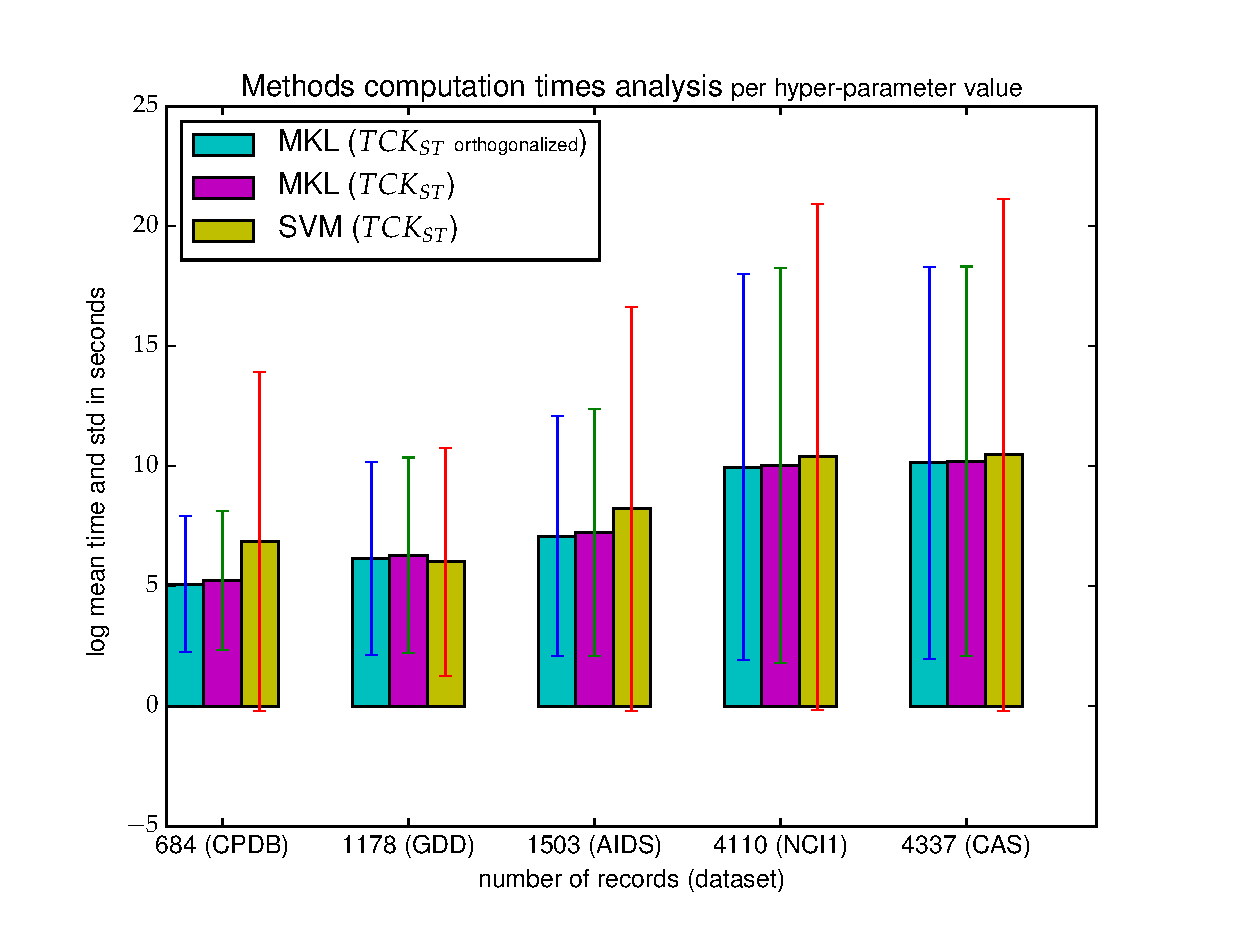
\includegraphics[scale=0.7]{Figures/method_times_avgstd}
    \caption{
        This plot shows the mean computation times among all the hyper-parameter values
        for the classifier, for each learning method and on all the benchmark datasets.
        Each plot shows the standard deviation among the same set of values plotted as well.
        The data here represented is taken from the experiments concerning the $TCK_{ST}$ kernel.
    }
        \label{fig:meantimes}
\end{figure}

\subsection{Analysis of model performances}

Here we present the empirical results we got from the devised experiments described
in the previous sections.
Data is divided in three tables, one for each of the three combinations we chose.
Each table reports the AUROC measure with the standard deviation measured with
a nested 10-fold cross validation.

Looking at Table \ref{table:results_st}, it is immediately evident how the results
obtained by our methodology are always comparable when not even better with respect
to the baselines except in when considering the GDD dataset which, as mentioned in
Section \ref{subsec:time_results} is a rather peculiar case given the smaller dimensions
of the parameters grid considered.
While the results for experiment 2 seem in accordance with the results in \cite{gmkl},
the $TCK_{ST}$ (experiment 3) performs significantly worse with our MKL method than with
the SVM.
(DRAFT: experiments 4 and 6 have unexpected high performancs though.)

Table \ref{table:results_stp} present results in accordance with Table \ref{table:results_st}
beside the case of GDD in which apparently the $ODD_{ST+}$ and the version with
contextual informations are able to outperform the baselines while maintaining
comparable performance when used in combination (experiment 1).

From these results something that we can infer is the scarce improvment gained from
using one kernel and its contextualized version in combination with or without
the orthogonalization of the feature space.
All the obtained results shows that either both kernel fare at the same level or
one of them dominates the combination outcome: section \ref{sec:kca} will cover
more in detail this aspect.

\begin{landscape}
%    \begin{table}[ht]
%        \label{table:times}
%        \caption{(DRAFT) Times}
%    \end{table}

    \begin{table}[ht]\footnotesize
        \centering
        \begin{tabular}{|l|l|r|r|r|r|r|}
            \hline
            n. &method&CAS&NCI1&AIDS&CPDB&GDD\\
            \hline
            1& $MKL~(ODDK_{ST}, TCK_{ST})^*$&0.9038 $\pm$ 0.0010&\textbf{0.9196 $\pm$ 0.0006}&0.8632 $\pm$ 0.0034&\textbf{0.8632 $\pm$ 0.0038}&0.8528 $\pm$ 0.0022\\
            2& $MKL~(ODDK_{ST})^*$&0.9033 $\pm$ 0.0010&0.9195 $\pm$ 0.0006&0.8627 $\pm$ 0.0035&0.8632 $\pm$  0.0029&0.8543 $\pm$ 0.0024\\
            3& $MKL~(TCK_{ST})^*$&0.9036 $\pm$ 0.0010&0.9189 $\pm$ 0.0006&\textbf{0.8634 $\pm$ 0.0034}&0.8625 $\pm$ 0.0032&0.8458 $\pm$ 0.0021\\
            \hline
            4& $MKL~(ODDK_{ST}, TCK_{ST})$&0.8960 $\pm$  0.0012&0.9076 $\pm$ 0.0007&0.8468 $\pm$ 0.0042&0.8517 $\pm$ 0.0034&0.8612 $\pm$ 0.0018\\
            5& $MKL~(ODDK_{ST})$&0.8899 $\pm$ 0.0013&0.8976 $\pm$ 0.0010 &0.8388 $\pm$ 0.0044&0.8401 $\pm$ 0.0033&0.8013 $\pm$ 0.0019\\
            6& $MKL~(TCK_{ST})$&0.8954 $\pm$ 0.0013&0.9095 $\pm$ 0.0006&0.8487 $\pm$ 0.0040&0.8525 $\pm$ 0.0030&0.8617 $\pm$ 0.0022\\
            \hline
             & $MKL~(ODDK_{ST})^{**}$&\textbf{0.9049 $\pm$ 0.0008}&0.9144 $\pm$ 0.0008&0.8515 $\pm$ 0.0031&0.8564 $\pm$ 0.0056&0.8498 $\pm$ 0.0026\\
             & $SVM~(ODDK_{ST})^{**}$&0.8982 $\pm$ 0.0017&0.9069 $\pm$ 0.0010&0.8262 $\pm$ 0.0052&0.8442 $\pm$ 0.0067&0.8473 $\pm$ 0.0038\\
            \hline
            7& $SVM~(TCK_{ST} + ODDK_{ST})$&0.9010 $\pm$ 0.0011&0.9110 $\pm$ 0.0011&0.8323 $\pm$ 0.0065&0.8497 $\pm$ 0.0072&0.8627 $\pm$ 0.0018\\
            8& $SVM~(TCK_{ST})$&0.9006 $\pm$ 0.0013&0.9150 $\pm$ 0.0011&0.8225 $\pm$ 0.0067&0.8422 $\pm$ 0.0080&\textbf{0.8674 $\pm$ 0.0026}\\
            \hline
        \end{tabular}
        \caption{\footnotesize AUROC results ($\pm$ standard deviation) relative
            to the $ODD_{ST}$ kernel and the $TCK_{ST}$ kernel. Results are
            obtained from a nested 10-fold cross validation. The first column is
            given as a reference to the experiment description given in Section
            \ref{sec:description}.
            The top part of the table contains the results of the main experiments
            while the bottom part those of the baselines.
            Lines marked with $^*$ refer to kernels whose feature space is orthogonalized
            according to the technique exposed in \ref{subsec:features}.
            Lines marked with $^{**}$ refer to results obtained in \cite{gmkl}.
        }
        \label{table:results_st}
        \medskip

        \begin{tabular}{|l|l|r|r|r|r|r|}
            \hline
            n. & metodo&CAS&NCI1&AIDS&CPDB&GDD\\
            \hline
            1& $MKL~(ODDK_{ST+}, TCK_{ST+})^*$&&&0.8632 $\pm$  0.0034&0.8632 $\pm$  0.0038&0.8528 $\pm$ 0.0022\\
            2& $MKL~(ODDK_{ST+})^*$&&&0.8628 $\pm$  0.0036&0.8652 $\pm$ 0.0030&\textbf{0.8720 $\pm$ 0.0021}\\
            3& $MKL~(TCK_{ST+})^*$&&&\textbf{0.8649 $\pm$  0.0030}&\textbf{0.8666 $\pm$  0.0038}&0.8711 $\pm$ 0.0018 \\
            \hline
            4& $MKL~(ODDK_{ST+}, TCK_{ST+})$&&&0.8468 $\pm$ 0.0042&0.8517 $\pm$ 0.0034&0.8612 $\pm$ 0.0018\\
            5& $MKL~(ODDK_{ST+})$&&&0.8489 $\pm$  0.0039&0.8461 $\pm$ 0.0036&0.8178 $\pm$ 0.0022\\
            6& $MKL~(TCK_{ST+})$&&&0.8503 $\pm$  0.0038&0.8528 $\pm$ 0.0039&0.8645 $\pm$ 0.0018\\
            \hline
            7& $SVM~(TCK_{ST+} + ODDK_{ST+})$&0.9022 $\pm$ 0.0015 &0.9163 $\pm$ 0.0011&0.8256 $\pm$ 0.0068&0.8521 $\pm$ 0.0038&0.8570 $\pm$ 0.0043\\
            8& $SVM~(TCK_{ST+})$&0.9008 $\pm$ 0.0017&0.9165 $\pm$ 0.0013&0.8222 $\pm$ 0.0067&0.8462 $\pm$ 0.0048&0.8588 $\pm$ 0.0028\\
            \hline
        \end{tabular}
        \caption{AUROC results ($\pm$ standard deviation) relative to the combination
                of the $ODD_{ST+}$ kernel with the $TCK_{ST+}$ kernel. Results are
                obtained from a nested 10-fold cross validation. Nomenclature and
                results disposition is analogue to the one of Table \ref{table:results_st}.}
        \label{table:results_stp}
    \end{table}

%    \begin{table}[ht]
%        \label{table:results_wl}
%        \caption{AUROC results ($\pm$ standard deviation) relative to the combination
%                of the $WL$ kernel with the $WLC$ kernel. Results are
%                obtained from a nested 10-fold cross validation. The nomenclature and
%            results disposition is analogue to the one of Table \ref{table:results_st}.}
%        \label{table:results_wl}
%    \end{table}
\end{landscape}

\section{Kernels Contribution Analysis}
\label{sec:kca}

%\begin{figure}[ht]
%    \centering
%    \includegraphics[scale=0.7]{Figures/weightdist}
%    \caption{(DRAFT: this plot is just an example of the available data for furhter analisys.
%        I think we may be mainly interested in the experiments were two kernels are combined
%        either with or without bucketization of the feature space.)
%        Kernel weight distributions for the $TCK_{ST}$ kernel
%    computed according to the full parameters grid, on the NCI1 dataset.
%    The $x$ axis shows all the employed kernel matrices indexed by their hyperparameters
%    values (ascending values left to right), the $y$ axis the weight values.
%    Each plot refers to one run of the nested 10-fold cross-validation routine relative to one
%    value for the $\Lambda$ parameter of EasyMKL. Weight values are the means between each of the inner
%    cross-validation runs. The vertical lines highlight the kernel with the maximum weight for each value of $\Lambda$.}
%        \label{fig:weightdist}
%\end{figure}


